\section{Problemi e Funzioni}

Ma cos'è un problema?\ Qualcosa del tipo:\ una domanda, con alcuni parametri da assegnare, ovvero una classe (non limitata) di domande, ciascuna delle quali vorremmo che avesse una risposta esatta e finita.

Nel nostro caso l'essenza di un problema è formalizzata come:
\begin{itemize}
    \item calcolare una funzione, oppure
    \item decidere l'appartenenza a un dato insieme.
\end{itemize}

\begin{definition}
    Siano $\Sigma, \Sigma_0, \Sigma_1$ alfabeti, con $\#, \triangleright \notin \Sigma_0 \cup \Sigma_1, \Sigma_0 \cup \Sigma_1 \subset \Sigma$, e $f:\Sigma_0^*\rightarrow\Sigma_1^*$ una funzione.\
    Allora si dice che una MdT $M=(Q,\Sigma,\delta, q_0)$ \textit{calcola} $f$, oppure che $f$ è \textit{Turing-calcolabile} o semplicemente \textit{T-calcolabile}, se e solamente se
    \[\forall w\in\Sigma_0^*, z\in\Sigma_1^* : f(w)=z\ \mathrm{se\ e\ solamente\ se}\ (q_0,\underline{\triangleright} w)\rightarrow_M^*(h,\triangleright z \underline{\#})\]
\end{definition}

\noindent In maniera del tutto analoga si definisce la nozione di \textit{\footnotesize WHILE}-calcolabilità.\

\begin{definition}
    Un comando $C$ \textit{calcola} $f:\mathit{Var}\rightarrow\mathbb{N}$, oppure $f$ è \textit{{\footnotesize WHILE}-calcolabile}, se e solamente se
    \[\forall \sigma \in \mathit{Var} \rightarrow \mathbb{N}:f(x)=n\ \mathrm{se\ e\ solamente\ se}\ \langle C,\sigma\rangle \rightarrow^*\sigma'\ \mathrm{e}\ \sigma'(x)=n\]
    (Si noti che la variabile $x$ viene usata per memorizzare sia il valore di ingresso che quello di uscita di $C$.)
\end{definition}

\begin{question}
    Ma se la $f$ fosse una funzione che opera su dati che non sono stringhe o memorie o numeri naturali?
\end{question}

\noindent Si supera la difficoltà per mezzo di opportune \textit{codifiche} dei dati, ovvero funzioni biunivoche che siano \textit{effettive} e \textit{facili}\footnote{Preciseremo in seguito cosa intendiamo per \textit{effettivo} e per \textit{facile}.\ Lo faremo considerando solo i numeri naturali, loro coppie ecc., quindi qui imbrogliamo un bel po', dando per buoni gli studi sull'argomento che si trovano in letteratura, e nella speranza di essere perdonati.}, nel modo seguente.

\begin{enumerate}
    \item Dato $x$ in formato $A$ codificalo come $y$ in formato $B$.
    \item Applica la MdT a $y$ e se e quando ottieni $z$ in formato $B$,
    \item traduci $z$ dal formato $B$ al formato $A$.
\end{enumerate}

\noindent Quindi con il rischio, ma non il timore, di banalizzare considereremo da qui in avanti solo i \textit{numeri naturali} come nostri dati; del resto lo abbiamo (quasi) già fatto nei linguaggi \textit{\footnotesize WHILE} e \textit{\footnotesize FOR}.

\begin{example}[Coda di colomba]

    La seguente funzione codifica coppie di naturali come un singolo naturale
    \[(x,y) \mapsto \frac{1}{2}\left(x^2+2xy+y^2+3x+y\right)\]
    ed è graficamente rappresentata come segue:

    \begin{figure}[H]
        \centering
        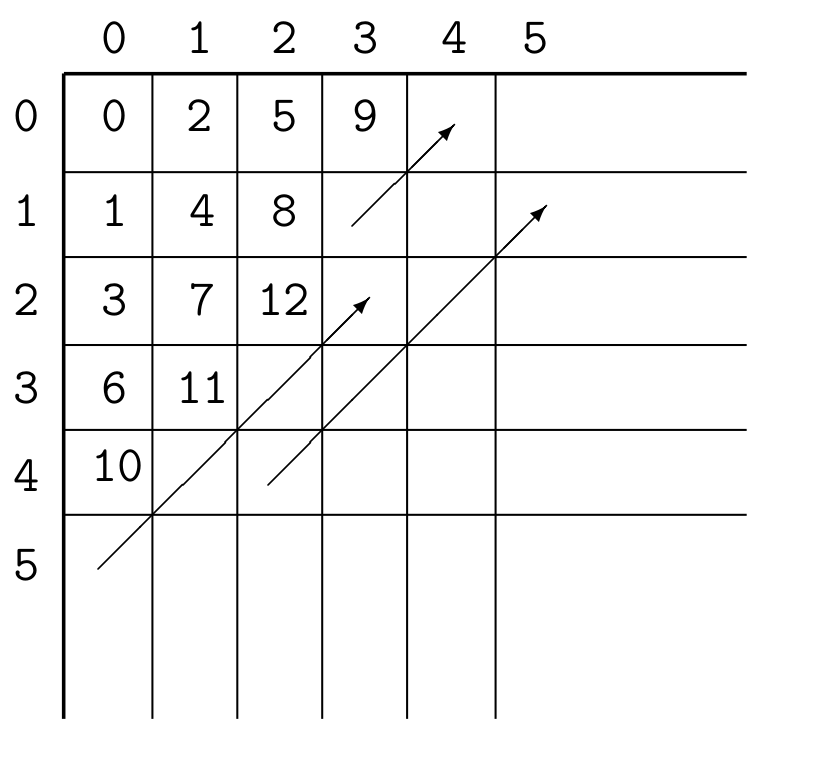
\includegraphics[width=0.4\textwidth]{codadicolomba}
    \end{figure}

    \noindent Risparmiamo al lettore sia la dimostrazione che questa funzione è biunivoca, sia lo sforzo per immaginare la funzione inversa, cioè la funzione di decodifica, che risulta essere definita così (si noti che nella colonna 0, l'elemento $n$-esimo è la somma dei primi $n$ naturali a partire da 1):
    \[n\mapsto\left(n-\frac{1}{2}k\times(k+1)\; , \; k-\left(n-\frac{1}{2}k\times(k+1)\right)\right)\]
    dove \[k=\left\lfloor{\frac{1}{2}\left(\sqrt{1+8\times n}-1\right)}\right\rfloor\]

\end{example}

\begin{definition}[Funzione totale]
    $f:A\rightarrow B$, sottoinsieme di $A \times B$ è una \textit{funzione totale} se e solamente se
    \begin{itemize}
        \item $\forall a \in A,\ \exists b\in B : (a,b) \in f$ (\textit{la funzione è definita ovunque})
        \item $(a,b), (a,c) \in f \Rightarrow b=c$ (\textit{unicità})
    \end{itemize}
\end{definition}

\noindent Vediamo adesso un esempio di funzione un po' strana, nella cui definizione si menziona la congettura di Goldbach, definita più sotto, che l'autore sottopose nel 1742 in una lettera all'attenzione di Eulero, il quale non rispose mai; tuttora non si sa se la congettura sia vera o meno e per il momento essa è stata verificata ``solo'' sui numeri fino a 400 miliardi.\
Ritorneremo su questa funzione per esaminare le relazioni che intercorrono tra funzioni e algoritmi.

\begin{example}{\label{Goldbach}}
    $gb : \mathbb{N} \rightarrow \mathbb{N}$
    \[gb(n) = \left\{\begin{array}{l l}
            1 & \mathrm{se\ la\ congettura\ di\ Goldbach\ \grave{e}\ vera} \\
            0 & \mathrm{altrimenti}                                        \\
        \end{array}\right.\]
\end{example}

\begin{definition}[Congettura di Goldbach]
    \[\forall m > 1\ \mathrm{si\ ha}\ 2m = p_1 + p_2\ \mathrm{con}\ p_1, p_2\ \mathrm{primi}.\]
\end{definition}

\begin{definition}[Funzione parziale]
    $f:A\rightarrow B$ è una \textit{funzione parziale} se è un sottoinsieme di $A \times B$ tale che
    \begin{itemize}
        \item $(a,b), (a,c) \in f \Rightarrow b = c$ (\textit{unicità}), ovvero esiste al più un $b \in B$ tale che $f(a)=b$
    \end{itemize}

    \noindent e quindi non si richiede che $f$ sia ovunque definita.
\end{definition}

\subsubsection{Notazione}

Data una funzione $f:A\rightarrow B$:

\begin{itemize}
    \item diremo che $f$ è \textit{definita} o \textit{converge} su $a$ (in simboli $f(a) \downarrow$) se $\exists b$ tale che $(a,b) \in f$ (cioè $f(a) = b$).
    \item altrimenti se $\nexists b$ tale che $(a,b)\in f$, diremo che $f$ non è definita o \textit{diverge} su $a$ ($f(a) \uparrow$).
\end{itemize}

\noindent Chiamiamo anche

\begin{itemize}
    \item \textit{dominio} di $f$ l'insieme $\{a\in A \; | \; f(a)\downarrow\}$ (coincidente con $A$ solo se $f$ è totale);
    \item \textit{codominio} di $f$ l'insieme $B$;
    \item \textit{immagine} (o \textit{range}) di $f$ l'insieme $\{b\in B \mid \exists a \in A : f(a)=b\}$.
\end{itemize}

\noindent Infine ricordiamo che

\begin{itemize}
    \item $f$ è \textit{iniettiva} se e solamente se $\forall a,b\in A.\ a\neq b$  implica $f(a)\neq f(b)$ (a volte nella terminologia nord-americana si dice che $f$ è uno-a-uno).
    \item $f$ è \textit{surgettiva} se e solamente se $\forall b \in B.\ \exists a \in A$ tale che $f(a)=b$ (ovvero se l'immagine e il codominio di $f$ coincidono).
    \item $f$ è \textit{biunivoca} se e solamente se è iniettiva e surgettiva.
\end{itemize}

\noindent (Si noti che la funzione iniettiva è invertibile sull'immagine.)

\vspace{12pt}

\noindent Abbiamo gli algoritmi, sia pure sotto forma di macchine di Turing o di programmi \textit{\footnotesize WHILE} e abbiamo le funzioni (non necessariamente T- o \textit{\footnotesize WHILE}-caclolabili).\
Allora siamo arrivati a porci una domanda cruciale.

\begin{question}
    Qual è il rapporto tra funzioni e algoritmi?
\end{question}

\noindent Una funzione $f$ è un insieme di coppie, cioè $f$ associa all'argomento il risultato senza dire \textit{come fare a calcolarlo}.\
Di conseguenza, \textit{non ci sono due funzioni diverse che per ogni argomento restituiscono lo stesso risultato}, il che riscritto in termini insiemistici si legge:\ \textit{non esistono due insiemi} diversi \textit{che hanno gli stessi elementi}!

Un algoritmo (quando c'è!) invece specifica \textit{come si calcola il risultato} a partire dall'argomento.\
In altre parole un algoritmo \textit{calcola} o \textit{rappresenta}, in modo \textit{finito}, una funzione.\
È facile vedere che ci possono essere più algoritmi che calcolano la stessa funzione --- saremo più precisi in seguito:\ qui basta considerare un programma \textit{\footnotesize WHILE} e aggiungergli un po' di \texttt{skip}.

Infine, riprendiamo la funzione $gb(n)$ dell'esempio \ref{Goldbach}.\
Non sappiamo a tutt'oggi se la congettura di Goldbach vale.\
Eppure un algoritmo per calcolarla esiste!\ ma non sappiamo quale esso sia, o meglio, quali essi siano:\ quelli che danno come risultato 1 per tutti gli ingressi, o quelli che danno sempre come risultato 1? \footnote{Gli intuizionisti rifiutano questo discorso:\ una entità matematica esiste se e solamente se la puoi costruire, e qui non esisterebbe (ancora)!\ Ciò che viene escluso è il \textit{tertium non datur} aristotelico.}

\medskip
\noindent Finalmente siamo arrivati al nocciolo:\

\begin{itemize}
    \item Quali sono le funzioni calcolabili?\ Per ora sappiamo quali sono le T-calcolabili e le \textit{\footnotesize WHILE}-calcolabili.
    \item Di quali proprietà godono?
    \item Esistono funzioni (totali/parziali), ovvero problemi, che non sono calcolabili?\ ovvero per cui si \textit{dimostra} che non esiste algoritmo che le calcoli?\ Tra questi problemi non calcolabili, ce ne sono di interessanti?
\end{itemize}

\noindent In questa prima parte del corso studieremo algoritmi e funzioni, con maggior attenzione alle seconde.\
In termini classici, l'enfasi sarà sugli aspetti \textit{estensionali}, perché ci occuperemo di ciò che è rappresentato (la semantica, il significato, la funzione) piuttosto di ciò che rappresenta (l'algoritmo, il programma):\ \textit{cosa si calcola}, piuttosto che come si calcola.\

La seconda parte del corso terrà invece in maggior considerazione gli algoritmi:\ \textit{come si calcola}.
